% START: alfred commands (Disheng)
\newcommand{\xpath}[1]{\mbox{\sf\small #1}}
%\newcommand{\htmlvalue}[1]{\mbox{\tt\small #1}}
\newcommand{\htmlvalue}[1]{\mbox{`#1'}}
\newcommand{\lc}[2]{\mbox{\ensuremath{LC(#1,#2)}}}%% local consistency
\newcommand{\gc}[2]{\mbox{\ensuremath{Sep(#1,#2)}}}%% global  consistency- separable now!

\newcommand{\allpages}{\mbox{\ensuremath{W}}}
\newcommand{\somepages}{\mbox{\ensuremath{Q}}}
\newcommand{\innersamples}{\mbox{\ensuremath{I}}}
\newcommand{\csample}{\mbox{\ensuremath{C}}}
\newcommand{\nil}[1]{\mbox{\ensuremath{nil_{}}}}
\newcommand{\accr}[1]{\mbox{\ensuremath{Acc(#1)}}}
\newcommand{\vect}[1]{\overrightarrow{#1}}
\newcommand{\rules}{\ensuremath{R}}
\newcommand{\allvects}{\ensuremath{\mathcal{V}^U}}
\newcommand{\allrules}{\ensuremath{\mathcal{R}}}
\newcommand{\nonallrules}{\ensuremath{\overline{\mathcal{R}}}}
\newcommand{\nonammrules}[1]{\ensuremath{\overline{\mathcal{R}}_{#1}}}
\newcommand{\ammvect}[1]{\ensuremath{V_{#1}}}
\newcommand{\ammrule}[1]{\ensuremath{R_{#1}}}
\newcommand{\nonammvect}[1]{\ensuremath{\overline{V}}_{#1}}
\newcommand{\allammrules}[1]{\ensuremath{\mathcal{R}_{#1}}}
\newcommand{\allammvalues}[2]{\ensuremath{\widehat{V}^{#1}_{#2}}}
\newcommand{\queryablevalues}[2]{\ensuremath{V^{#1}_{#2}}(U)}
\newcommand{\lqueryablevalues}[3]{\ensuremath{V^{#1}(#2,#3)}}
\newcommand{\ltypedqueryablevalues}[4]{\ensuremath{V_{#1}^{#2}(#3,#4)}}
\newcommand{\typedqueryablevalues}[2]{\ensuremath{V_{#1}(#2)}}
\newcommand{\equivalence}[1]{\ensuremath{Eq_{U}(#1)}}

\newcommand{\lessexpressive}[1]{\ensuremath{Exp_{min}{(#1)}}}
\newcommand{\equivalencerules}[3]{\ensuremath{Eq^{#3}(#1,#2)}}

\newcommand{\subtypeof}{\ensuremath{\subseteq}}
\newcommand{\supertypeof}{\ensuremath{\supseteq}}

\newcommand{\mq}{\mbox{\em MQ}}
\newcommand{\alf}{\mbox{\sc alf}}
\newcommand{\alfrex}{\mbox{\sc AlfREX}}
\newcommand{\sampler}{{\sc Page\-Sampler}}
\newcommand{\page}{\mbox{\em w}}
\newcommand{\att}[1]{\mbox{\sf #1}}
\newcommand{\val}[1]{{\mbox{\sf '#1'}}}
\newcommand{\valm}[1]{\mbox{\sf #1}}
\newcommand{\abs}[2]{\mbox{\sf abs(#1,#2)}}
\newcommand{\rel}[2]{\mbox{\sf #1(`#2')}}
%\newcommand{\lab}[1]{\mbox{\ensuremath{l(#1)}}}

\newcommand{\alg}[1]{{\sc #1}}
\newcommand{\scegliDomanda}{\textsc{choose\-Question}}
\newcommand{\terminaAlgoritmo}{\mbox{\textsc{halt}}}
\newcommand{\espandiBacinoRegoleCandidate}{\textsc{expandRuleSet}}
\newcommand{\leggiRisposta}{\mbox{\textsc{oracle}}}

\newcommand{\type}[1]{\mbox{\em \ensuremath{#1}}}

\newcommand{\dalvi}{DBLP:journals/pvldb/DalviKS11}
\newcommand{\mdl}{DBLP:journals/corr/math-ST-0406077}
\newcommand{\lixto}{DBLP:conf/pods/GottlobKBHF04}
\newcommand{\angluin}{DBLP:journals/tcs/Angluin04}
\newcommand{\myjacm}{DBLP:journals/jacm/CrescenziM04}
\newcommand{\SL}{DBLP:journals/tnn/Vapnik99}
\newcommand{\srm}{DBLP:journals/tit/Shawe-TaylorBWA98}
\newcommand{\ALsurvey}{settles.tr09}

%\newtheorem{example}{Example}

% END %

%\section{Wrapper Generation}
Detecting rules to extract the subject-object pairs related to a property $p$ is the most difficult step when aiming to extract \ac{RDF} from templated website.
Here, we present our current implementation of the wrapper induction module interface of REX, which aims to extract subject-object pairs for $p$ from a set of pages $\allpages$ that belong to the same website and share a common template.
We assume that an \emph{example generator} provides the input set ${\examples}$ containing a subset of the pairs that can be extracted from the pages in $\allpages$. 
Formally,  let $\somepages$ denote the set of pages that contain a pair in $\examples$:
\begin{equation}
 \somepages = \{\page: \page \in \allpages,\ (s, o)\in {\examples} \wedge (\lab{s},\lab{o}) \in\ \page\},
\end{equation}
where  $(\lab{s},\lab{o}) \in \page$ denotes that at least one of the labels of $s$ and at least one of the labels of $o$ occur in the page $\page$. %In other words, 
We use the pairs in ${\examples}$ to gain the positive annotations for the pages in $\somepages$. These  annotations are needed to automatically infer a set of wrappers, i.e., a set of extraction rule pairs that extract the target subject-object pairs.

%Inferring a wrapper from a large number of annotations increases the computational costs. On the other hand, 
%the accuracy of the generated wrappers strongly depends on the number of training annotations used in the inference process.
%With a small number of annotations, the generated wrappers could be biased towards the variants of the HTML template observable in the sampled pages. For example, if the triples in $\somepages$ are all about famous actors, it might be the case that the inferred rules do not work on pages related to less popular actors in $\allpages$, since these pages could obey a slightly different variant of the template without some fields such as the prizes won, the user comments, etc. etc.

%We introduce a technique that first generate a set of wrappers %starting from a small set of annotations to reduce the costs, and %then rank the wrappers' rules using all the pairs extracted from %$\somepages$ to cover a large
%number of template variants.


% in alternativa alcuni sistemi supervisionati come ALF possono migliorare e certificare la qualità
% la copertura delle regole inferite
To avoid the extraction of incorrect values, our approach includes a technique to evaluate the output wrapper coverage, i.e., the number of pages in {\allpages} for which the wrappers inferred from {\somepages} correctly extract the target subject-object pairs. 

%\subsubsection{Learning Web Wrappers}
%\label{sec:learning-wrappers}

Listing~\ref{lst:learning-wrappers} reports the pseudo-code of our algorithm to generate the wrappers that extract subject-object pairs related to a property $p$ from a set of pages: 
%
it takes as input the set of pages $\allpages$ and the set of examples ${\examples}$.
%, i.e., the pairs $(s,o)$ generated by the previous component, the \emph{example generator}. 
To abstract the extraction rules generative process in our implementation, we assume that there exists, as a parameter of the algorithm, a class of all the creatable extraction rules $\allrules$. It corresponds to the set of XPath expressions that we can generate over the pages in \allpages.

\begin{algorithm}[htb!]
\caption{{\alfrex}: Extract subject-object pairs from a website.}\label{lst:learning-wrappers}
\label{alg:alfrex}
\begin{algorithmic}[1]
\renewcommand{\algorithmicensure}{\textbf{Output:}}
\newcommand{\LET}{\mbox{\textbf{let}}}
\renewcommand{\algorithmicrequire}{\textbf{Input:}}
\REQUIRE \ac{KB} $K$, a predicate $p$, a set of examples $\examples = \{(s,o)|(s,p,o) \in K\}$
\REQUIRE a set of pages $\allpages=\{w_1,\ldots,w_{|\allpages|}\}$ containing data w.r.t. predicate $p$

\renewcommand{\algorithmicrequire}{\textbf{Parameter:}}
\REQUIRE a class of extraction rules $\allrules$ over $\allpages$
\REQUIRE $k$, the number of sample pages for generating the rules

\ENSURE set $T$ of pairs of strings extracted from pages $W$
\bigskip
\STATE $T := \emptyset$; {\em // output pairs of strings}
\STATE $Q := \{\page \in \allpages$: $(\lab{s},\lab{o}) \in \page$, $ (s, o) \in \examples\};$\label{lst:Q}
\STATE $I :=$ a set of $k$ random pages from $Q$;\label{lst:I}
\STATE $R_s := \{r, r \in \allrules, \page \in I, (\lab{s}, \lab{o}) \in \page, r(\page) = \lab{s}\}$;\label{lst:Rs}
\STATE $R_o := \{r, r \in \allrules, \page \in I, (\lab{s}, \lab{o}) \in \page, r(\page) = \lab{o}\}$;\label{lst:Ro}
\STATE $(r_s, r_o) := \argmax_{r_s\in R_s, r_o \in R_o}$~~$|\{\page, \page \in Q, (\lab{s},\lab{o}) \in \page,$\\$ r_s(q) = \lab{s}\ \AND\ r_o(q) = \lab{o}\}|$;\label{lst:best-pair}
\STATE $\{r_s^1,r_s^2,\ldots, r_s^n\} \leftarrow \{r, r \in R_s, r(Q)=r_s(Q) \}$;\label{lst:best-vector-s}
\STATE $\{r_o^1,r_o^2,\ldots, r_o^m\} \leftarrow \{r, r \in R_o, r(Q)=r_o(Q) \}$;\label{lst:best-vector-o}

\FOR{$q\in \allpages$}\label{lst:forall-start}
    \IF {($r_s^1(q)=\ldots=r_s^n(q)\ \AND\ r_o^1(q)=\ldots=r_o^m(q)$)}\label{lst:check}
    \STATE $T \leftarrow T \cup \{(r_s^1(q),r_o^1(q))\}$;
    \ENDIF
\ENDFOR\label{lst:forall-end}

\RETURN $T$;

\end{algorithmic}
\end{algorithm}


As a first step (line~\ref{lst:Q}), the algorithm computes the set of pages $Q$
(we assume $Q \neq \emptyset$).
Then, it picks up a small set of sample pages $I$ from $Q$.%
In our implementation, we set $k = |I| = 10$.
%
From the pages in $I$ two initial sets of extraction rules, $R_s$ and $R_o$, are generated (lines~\ref{lst:Rs}-\ref{lst:Ro}), as follows. 
%
%
First, we analyze the DOM tree of the pages to locate nodes that are part 
of the template. We use these nodes as roots of XPath expressions that 
match with the input pair. To discover the template nodes, we compute the occurrences of the textual leaf nodes in the pages. Following the intuition developed in~\cite{exalg}, 
we consider template nodes the document root, the nodes with an {\em id} attribute, 
and  the text leaves that occur exactly once  with same value and same root-to-leaf sequence of tags in a significant 
percentage (80\%) of pages.  The rationale is that it is very unlikely that a node occurs exactly once in several pages with the same root-to-leaf path by chance; rather, it is likely repeated  in every page since it comes from a piece of the underlying HTML template.

Template nodes are then used as {\em pivot nodes} to generate XPath expressions that 
match with nodes containing a textual leaf that equals the subject (object) of the 
input pair. Given a pivot node $l$, an XPath expression for the textual node $t$ 
is computed by appending three expressions: $(i)$~an expression that matches with the
pivot node $t$, $(ii)$~the path from $t$ to the first ancestor node,
$n_{lt}$, shared by $t$ and $l$, $(iii)$~the path from $n_{lt}$ to $l$ 
(which descends from the shared ancestor node to the target textual node).
To avoid an excessive proliferation of rules, we bound the length of
the XPath expressions, i.e., the number of XPath steps.
We observed that producing rules longer than 8 steps do not produce any benefit.

\begin{figure*}[htb]
\newcommand{\sxpath}[1]{\xpath{\scriptsize#1}}
\begin{tabular}{ccc}
\multicolumn{3}{c}{
\vspace{0pt}
    \resizebox{0.95\textwidth}{!}{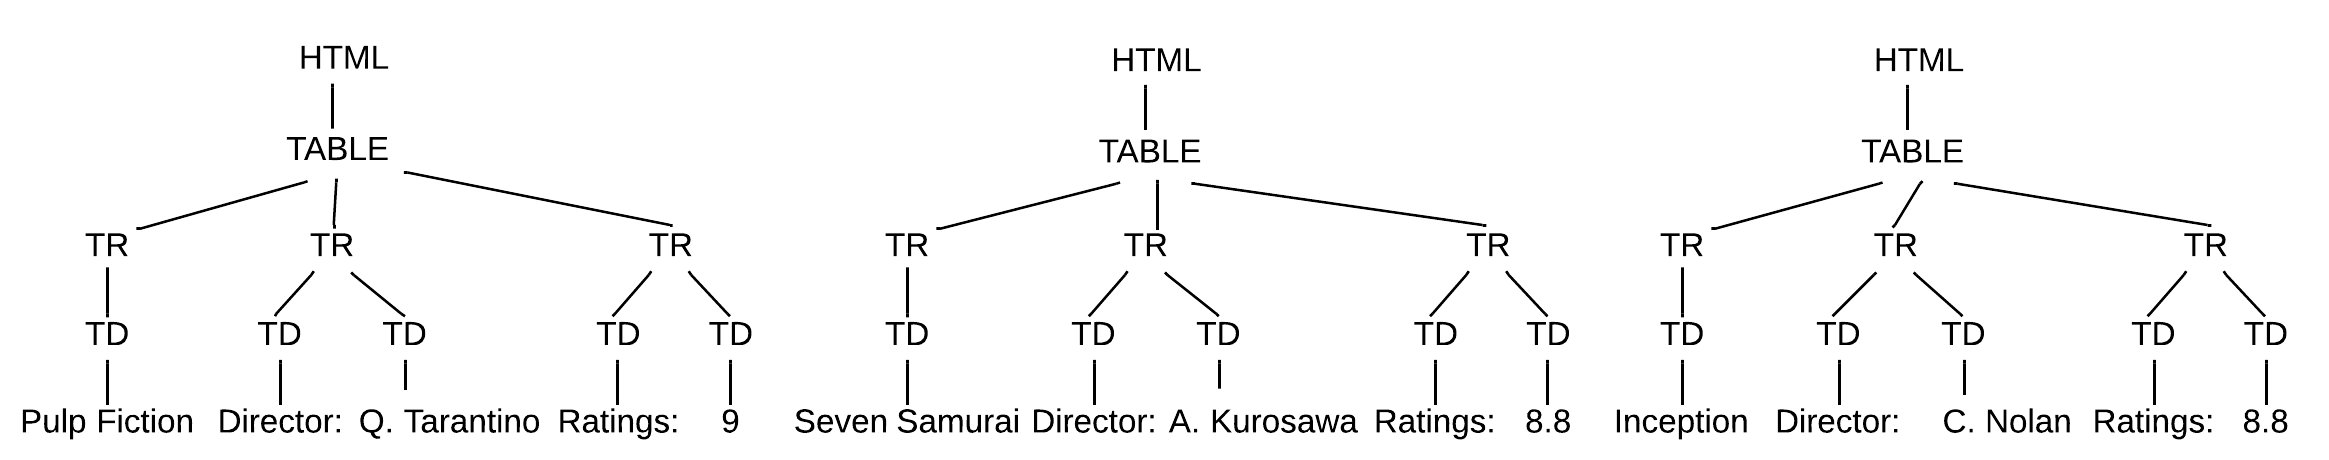
\psfig{file=part_02/semi_structured_annotation/ISWC_REX/dom-I.png}}
}\\
%
\multicolumn{3}{c}{\bf (a)}\\
%
\multicolumn{1}{c}{
    \resizebox{0.2\textwidth}{!}{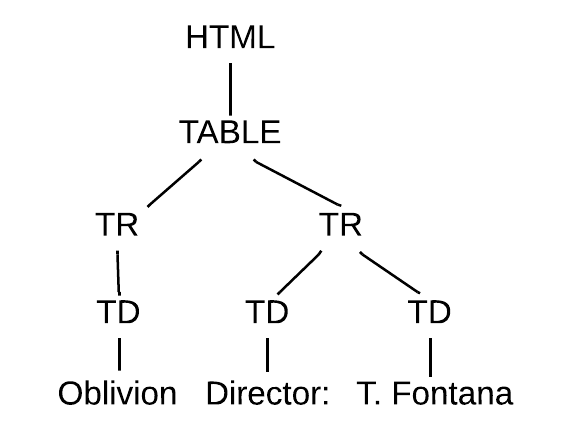
\psfig{file=part_02/semi_structured_annotation/ISWC_REX/dom-Q.png}} 
} &
\multicolumn{1}{@{}c@{}}{
    \raisebox{0.5\totalheight}{
    \scalebox{0.75}{
\begin{tabular}{@{}r@{:~}l@{}}
\multicolumn{2}{l}{\em Extraction rules}\\
$r^1$  & {\sxpath{//*[contains(.,"Ratings:")]/../p-s::tr[2]/td/text()
}}\\
$r^2$  & {\sxpath{//*[contains(.,"Director:")]/../p-s::tr[1]/td/text()
}}\\
$r^3$  & {\sxpath{/html/table/tr[1]/td/text()}}\\
\multicolumn{2}{l}{\em ps = preceding-siblings} \\
\end{tabular}}}}  &
\vspace{0pt}
    \resizebox{0.35\textwidth}{!}{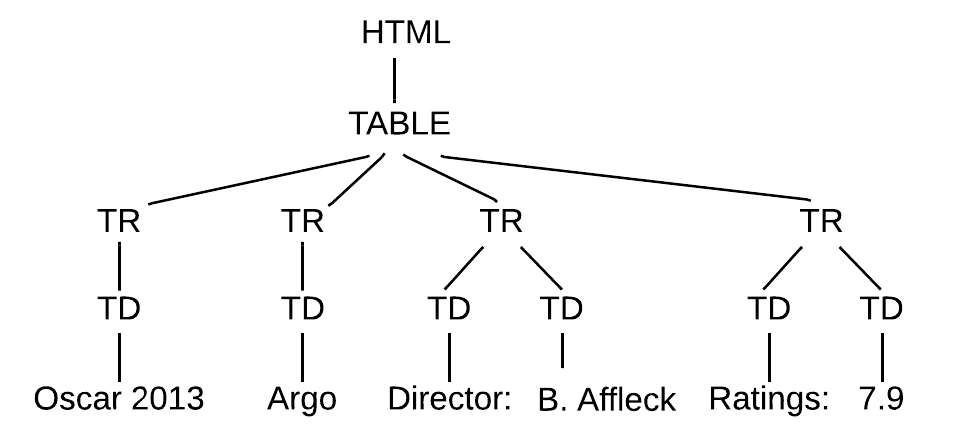
\psfig{file=part_02/semi_structured_annotation/ISWC_REX/dom-W.png}} \\
%
\multicolumn{1}{c}{\bf (b)} & \multicolumn{1}{c}{\bf (c)} & \multicolumn{1}{c}{\bf (d)} 
\\
\end{tabular}
 \caption{%
 {\bf (a)} DOM trees of three pages (in a fictional set $I$), 
 {\bf (b)} a page in $Q$ (with a template that differs from those of the pages in $I$), 
 {\bf (c)} some rules to extract the movie title, and
 {\bf (d)} a page in $W$ (with a template that differs from those of the pages in $Q$).}%
 \label{fig:dom-trees}
\end{figure*}


The above step produces several extraction rules that correctly work on the pages 
in $I$. However some of these rules could not work on a larger set of pages. 
For example, consider a set of pages such as those shown in Figure~\ref{fig:dom-trees} (a). Assuming that the leaf nodes {\htmlvalue{Director:}} and {\htmlvalue{Ratings:}} appear once with the same root-to-leaf path in most of the pages in $I$, they would be considered as template nodes. Figure~\ref{fig:dom-trees} (c) reports an example of the XPath expressions pivoted in these nodes, and generated to extract the movie title.
%
%\end{example} 
%
Notice, however, that rule $r^1$ does not extract the movie title on pages like that depicted in Figure~\ref{fig:dom-trees} (b), i.e., pages without user ratings.
To improve the accuracy of the rules generated from pages in $I$, we evaluate the generated rules over $Q$, and select those that extract the largest number of annotations (line~\ref{lst:best-pair}). In our example, the extraction rules $r^2$ and $r^3$ would be selected, while $r^1$ would be discarded, as the former rules work also on the page of Figure~\ref{fig:dom-trees} (b), while the latter does not. 

%\floatname{algorithm}{Listing}



The selected rules are those better working for the pages in $Q$, that are the pages containing pairs of $K$. Although it is likely that these rules also work for the whole collection of input pages, it might also be the case that {\allpages} contains pages obeying to a slightly different template not observed within $Q$. For example, consider the page in Figure~\ref{fig:dom-trees} (d): since the movie has been awarded 3 Oscars, the corresponding page has small structural differences, and neither $r^1$ nor $r^3$ correctly extract the title. 


To overcome this issue, we leverage the redundancy of equivalent rules generated in the above steps. Targeting only resources from pages for which the extraction is likely to work correctly, we return the pairs (lines~\ref{lst:best-vector-s}-\ref{lst:best-vector-o}) on which all the distinct yet equivalent rules return the same value. Again from our example, observe that rules $r^2$ and $r^3$ extract different values from the page in Figure~\ref{fig:dom-trees} (d) ({\em Argo} and {\em Oscar 2013}, respectively), therefore, none of the values extracted from that page would be added in the final output. 
%{\bf DQ: cosi funziona? :)}
%{\bf DA SISTEMARE. ATTENZIONE: L'ESEMPIO NON FUNZIONA LE DUE REGOLE SI COMPORTANO ALLO STESSO MODO}
All these rules are used later (lines~\ref{lst:forall-start}-\ref{lst:forall-end}) to check that they extract the same value (line~\ref{lst:check}) from a web page.


%We could also rely to other supervised systems (such as~\cite{DBLP:conf/www/CrescenziMQ13a}) to further improve and guarantee the quality and the coverage of the extraction rules.

